\clearpage
\chapter{CP violation with the Hyper-Kamiokande experiment}
\label{cha:cp_hk}
%\chapter{Hyper-Kamiokande sensitivity to $\delta_\text{CP}$}

The violation of the CP--symmetry is a well-known process in the quark sector of the standard model (SM),

[explain what CP transoformation on a field is]

C and CP violation are some of the conditions required in order to generate %
an asymmetry between matter and antimatter particles, together with %
baryon number violation and interactions out of thermal equilibrium~\cite{Sakharov:1967dj}.
%The observed baryon asymmetry in our Universe amounts to~\cite{Tanabashi:2018oca, Aghanim:2018eyx}
%\begin{equation*}
%	\eta = \frac{n_{B}}{n_\gamma}\quad,\quad \np{5.8e-10} \leq \eta \leq \np{6.6e-10}\quad\text{at}\ 95\% \text{C.L.}
%\end{equation*}
The amount of CP violation in the quark sector is not enough %
to describe the observed baryon asymmetry within the SM.
An asymmetry in the lepton sector, however, could be translated into baryogenesis, %
via non-perturbative sphaleronic processes~\cite{Fukugita:1986hr}.
This process, called \emph{leptogenesis}, would be allowed by the addition of %
right-handed Majorana neutrinos to the SM, which can violate lepton number.
This elegant solution to explain the baryon asymmetry is a strong motivation %
for searches of signals of CP violation in the lepton~sector.


It has been extensively observed~\cite{Christenson:1964fg,Aubert:2001sp, Abe:2001xe, Aaij:2013iua, Aaij:2019kcg}, %
giving clear evidence that the Cabibbo-Kobayashi-Maskawa (CKM) matrix is complex.
The CKM matrix arises from mixing of quarks in charged-current interactions (see \refeq{eq:real_quark_cc}), %
when describing the fermion fields in the mass basis.

It is a generic $N \times N$ unitary matrix, where $N$ is the number of fermion generations.
The $N^2$ independent real parameters which describe the matrix are typically categorised into 
\begin{align*}
	\frac{N(N-1)}{2} &\quad \text{mixing angles} \\
	\frac{N(N+1)}{2} &\quad \text{phases}\ ,
\end{align*}
even though, not all the phases are observables, or give physical effects.
Excluding the CC term, the SM Lagrangian is invariant under a global phase transformation %
of the quark fields, such as
\begin{equation}
	q_\alpha^{U,D} \longmapsto e^{i \phi_\alpha^{U,D}} q_\alpha^{U,D}\ .
\end{equation}
Applying this to the CC Lagrangian of \refeq{eq:real_quark_cc}, we can factorise %
a common phase outside:
\begin{align*}
	%\label{eq:real_quark_cc}
	j^\mu_\text{CC,Q}&= 2 \sum_{\shortstack{$\scriptstyle \alpha = u, c, t$ \\ $\scriptstyle \beta = d, s, b$}} %
			    \cj{q}^U_{L\alpha}\, \gamma^\mu e^{-i\phi_\alpha^U} \, V_{\alpha \beta}\, e^{i \phi_\beta^D} q^D_{L\beta} \\
			 &= 2 e^{-i (\phi_t^U - \phi_b^D)} \sum_{\shortstack{$\scriptstyle \alpha = u, c, t$ \\ $\scriptstyle \beta = d, s, b$}} 
			    \cj{q}^U_{L\alpha}\, \gamma^\mu e^{-i(\phi_\alpha^U-\phi_t^U)} \, V_{\alpha \beta}\, %
			    e^{i (\phi_\beta^D-\phi_b^D)} q^D_{L\beta}\ ,
\end{align*}
showing that there are $2 N -1$ phases that can be reabsorbed in a redefinition of the fields.
A common rephasing would leave the charged current unchanged.
It follows that the physical phases are
\begin{equation}
	\frac{N(N+1)}{2} - 2N +1 = \frac{(N-1)(N-2)}{2}
\end{equation}
and the total physical parameters are
\begin{equation}
	\frac{N(N-1)}{2} + \frac{(N-1)(N-2)}{2} = (N-1)^2
\end{equation}
In the case of three generations, there are four physical parameters, divided %
amongst three angles and one complex phase.
The complex phase is responsible for CP violation.
From a model building point of view, the complex phase may arise from complex Yukawa couplings %
and/or from a relative CP-violating phase in the vacuum expectation values of Higgs fields.

As three generations exist also in the lepton sector, %
an entirely analogous phase is expected in mixing matrix of lepton mass.
The~best probe to discovery CP violation is neutrino oscillation, being a purely weak process in which %
\mbox{CP--con}\-ju\-gate processes can be easily studied.

CP violation in the leptonic sector is plausible and it is also a necessary ingredient for leptogenesis.
Neutrino oscillation experiments can lead to the discovery of CP violation, and it is %
foreseen that HK will determine the value of~$\delta_\text{CP}$, %
a milestone which requires precise measurements and a deep understanding of the systematic errors.


\section{CP violation in neutrino oscillations}
\label{sec:cp_oscillation}

The Pontecorvo--Maki--Nakagawa--Sakata (PMNS) matrix, is usually parameterised as in \refeq{eq:pmns}, %
with the addition of two more phases if the neutrino is Majorana.
The PMNS matrix relates flavour states $\alpha = e, \mu, \tau$ with mass eigenstates $i = 1, 2, 3$  %
as $\ket{\nu_\alpha} = \sum_i U^*_{\alpha i} \ket{\nu_i}$.
The probability of flavour oscillation in vacuum is hence computed as
%$P(\nu_\alpha \to \nu_\beta)$ is computed as $\qty|\mel{\nu_\alpha}{e^{-i\mathcal{H}t}}{\nu_\beta}|^2$ %
\vspace{-0.4em}
\begin{equation}
	P(\nu_\alpha \to \nu_\beta) \equiv \qty|\mel{\nu_\alpha}{e^{-i\mathcal{H}t}}{\nu_\beta}| ^2 = %
	\sum_{ij} U_{i\alpha}^* U_{\beta i} U_{\alpha j} U_{j\beta}^* %
	\exp \qty(-i \frac{\Delta m_{ij}^2 L}{2 E})\ ,
\vspace{-0.4em}
\end{equation}
where $\mathcal{H}$ is the Hamiltonian, $t \simeq L$ and $\Delta m^2_{ij} = m_i^2 - m_j^2$, %
and it depends on the physical angles and phases of the PMNS matrix, %
with the exception of the Majorana phases $\gamma_{1,2}$.
The~\mbox{CP--con}\-jugate of a neutrino with negative helicity is an antineutrino with positive helicity, %
which, in terms of neutrino oscillations, means transforming the $\nu_\alpha \to \nu_\beta$ oscillation channel %
into the $\cj{\nu}_\alpha \to \cj{\nu}_\beta$ channel.
The violation of CP in neutrino oscillation can be quantified by the asymmetry in oscillation probabilities %
between neutrinos and antineutrinos, which in vacuum reads as
\vspace{-0.5em}
\begin{equation}
	\label{eq:asymmetry}
	A^\text{CP}_{\alpha\beta} = P(\nu_\alpha \to \nu_\beta) - P(\cj{\nu}_\alpha \to \cj{\nu}_\beta) = %
	4 \sum_{i>j}\imaginary\qty[U_{i\alpha}^* U_{\beta i} U_{\alpha j} U_{j \beta}^*] \sin\qty(\frac{\Delta m_{ij}^2 L}{2E})\ .
\vspace{-0.3em}
\end{equation}
%with $t \simeq L$ and $\Delta m^2_{ij} = m_i^2 - m_j^2$.
The quartic product $U_{i\alpha}^* U_{\beta i} U_{\alpha j} U_{j \beta}^*$ wich $\alpha\neq\beta$ %
and $i \neq j$ is a physical observable and so it is invariant under a reparameterization of the mixing matrix.
The imaginary part of the quartic products is antisymmetric on the indices $\alpha,\beta$ and $i, j$ and %
they are all equal up to a sign.
We can prove this by starting with the unitarity of the mixing matrix, for example $U\,U^\dagger = 1$,
\begin{equation}
	\sum_{i=1}^3 U_{\alpha i} U_{\beta i}^* = \delta_{\alpha\beta} 
\end{equation}
and multiplying it by $U_{\alpha j}^* U_{\beta j}$.
We can write the new relation as
\begin{equation}
	|U_{\alpha j}|^2 |U_{\beta j}|^2 + \sum_{i\neq j} U_{\alpha i} U_{\beta j} U_{\beta i}^* U_{\alpha j}^* = %
		\delta_{\alpha\beta} |U_{\alpha j}|^2\ ,
\end{equation}
and by taking the imaginary part of left-hand and right-hand sides of the equation it follows that
\begin{equation}
	\sum_{\alpha \neq \beta} \imaginary\qty[U_{\alpha i} U_{\beta j} U_{\beta i}^* U_{\beta j}^*] = 0\ .
\end{equation}
This condition and the anti-symmetry of the indices reveal that th quartic product are all equal up to a sign.
This value is called \emph{Jarlskog invariant} and using the parametrisation of the PMNS matrix in Eq.~\ref{eq:pmns} %
it is equal to~\cite{Jarlskog:1985ht}
\begin{equation}
	\label{eq:jarlskog}
	J = \imaginary\qty[U_{\mu 3} U_{e 2} U_{\mu 2}^* U_{e 3}^*] = %
	    \frac{1}{8} \cos\theta_{13} \sin(2\theta_{12}) \sin(2\theta_{13}) \sin(2\theta_{23}) \sin \delta_\text{CP}\ .
\end{equation}
It follows that CP violation can only be measured in ``appearance'' channels, as %
the argument of the imaginary part of Eq.~\ref{eq:asymmetry} is real for $\alpha = \beta$. % and so $A^\text{CP}_{\alpha\alpha} = 0$.
For example, for the main channel of interest for long beaseline experiments (LBL), $\nu_\mu \to \nu_e$, %
the asymmetry looks like:
\begin{align}
	\mathcal{A}_{\mu e}^\text{CP} =&\ \frac{1}{2} \cos\theta_{13} \sin(2\theta_{12}) %
		\sin(2\theta_{13}) \sin(2\theta_{23}) \sin \delta_\text{CP} \notag \\
		&\times \qty[\sin \Delta_{12} - \sin \Delta_{13} + \sin \Delta_{23}]\ ,
\end{align}
where $\Delta_{ij} = \flatfrac{\Delta m_{ij}^2 L }{4 E}$.
Because of the above discussion, all the CP asymmetries, measured on each channel, are equal up to a sign:
\begin{equation}
	\mathcal{A}_{\mu e} = \mathcal{A}_{\tau \mu} = \mathcal{A}_{e \tau} = %
	- \mathcal{A}_{e \mu} = - \mathcal{A}_{\mu \tau} = - \mathcal{A}_{\tau e}  \ .
\end{equation}
Including matter effects, we can focus on the limit where the effects of the atmospheric mass difference dominates.
This holds to LBL experiments and leads to helpful cancellations in the evolution equation which reads
\begin{equation}
	i \dv{}{x} \mqty(\psi_{\alpha 1} \\ \psi_{\alpha 2} \\ \psi_{\alpha 3}) =
		\frac{1}{2E} \mqty (s_{13}^2 \Delta m_{31}^2 + a & 0 & c_{13} s_{13} \Delta m_{31}^2 \\
				    0				 & 0 &  0			     \\
				    c_{13} s_{13} \Delta m_{31}^2 & 0 & c_{13}^2 \Delta m_{31}^2) %
				    \mqty(\psi_{\alpha 1} \\ \psi_{\alpha 2} \\ \psi_{\alpha 3})\ ,
\end{equation}
which depends only on the mixing angle $\theta_{13}$ and is independent of the CP-violating phase.
Hence, CP violation is not observable in experiments which are only sensitivite to $\Delta m_{31}^2$, %
just by looking at neutrino oscillations in matter, as well as in vacuum.
This is easily understandable, as the limit dictated by \refeq{eq:hierarchy} corresponds to an effective %
two-flavour oscillation.
However, the oscillation probabilities of neutrinos and antineutrinos in matter are not the same, %
because the medium is not CP-invariant and it induces CP violation in the oscillation probabilities.
\iffalse
\begin{align}
	P(&\nu_\mu \to \nu_e) = %
	\ 4 c_{13}^2 s_{13}^2 s_{23}^2\,\sin^2 \Delta_{31}^2\notag  \\
	&\ + 8 c_{13}^2 s_{12} s_{13} s_{23}\, (c_{12} c_{23}\, \uj{\cos\delta_\text{CP}} -s_{12}s_{13}s_{23}) %
	\,      \cos\Delta_{32} \sin \Delta_{31} \sin\Delta_{21}\notag  \\
	&\ - 8 c_{13}^2 c_{12} c_{23} s_{12} s_{13} s_{23}\, \uj{\sin\delta_\text{CP}} %
	\sin\Delta_{32} \sin \Delta_{31} \sin\Delta_{21} \notag \\
	&\ + 4 s_{12}^2 c_{13}^2\,(c_{12}^2 c_{23}^2 + s_{12}^2 s_{13}^2 s_{23}^2 - %
	2c_{12}c_{13} s_{12} s_{23} s_{13}\,\underline{\cos\delta_\text{CP}}) \sin^2\Delta_{21} \notag \\
	&\ - 8 c_{13}^2 s_{13}^2 s_{23}^2 \qty[\frac{aL}{4 E} (1-2s_{13}^2) \cos\Delta_{32} \sin\Delta_{31} %\\
	- \frac{a}{\Delta m_{31}^2} (1-2s_{13}^2) \sin^2\Delta_{31}]\ ,
\end{align}
where $s_{ij} = \sin \theta_{ij}$, $c_{ij} = \cos\theta_{ij}$,
and $a = 2\sqrt{2} G_F\,n_e\,E$ embeds matter effect with $n_e$ the electron density of the medium.
\fi

The effect of the CP--violating phase on the asymmetry of Eq.~\ref{eq:asymmetry} can be appreciated from the plot in Fig.~\ref{fig:mass}.

\begin{figure}
	\begin{minipage}[t]{0.44\textwidth}
		\centering
		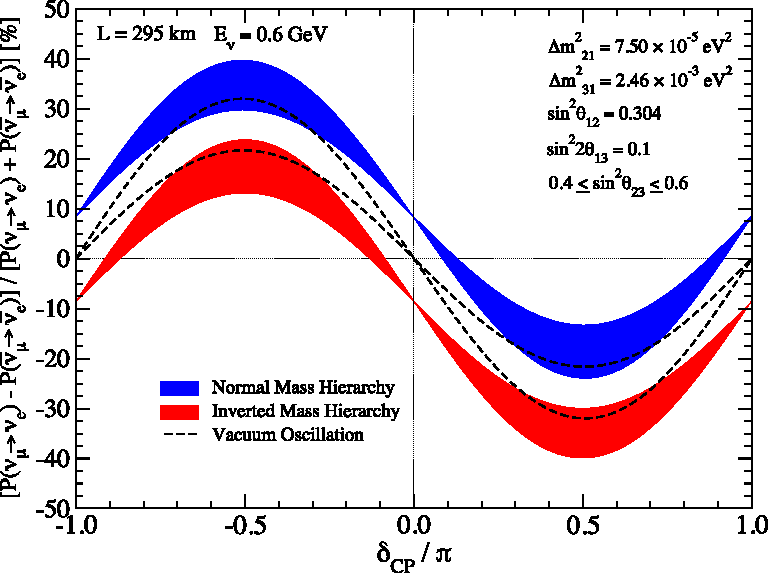
\includegraphics[width=\linewidth]{CPsensitivityHKDR.pdf}
		\captionof{figure}{Effect of $\delta_\text{CP}$ on the normalised asym\-metry from Eq.~\ref{eq:asymmetry}.}
		\label{fig:mass}
	\end{minipage}
	\hfill
	\begin{minipage}[t]{0.52\textwidth}
		\centering
		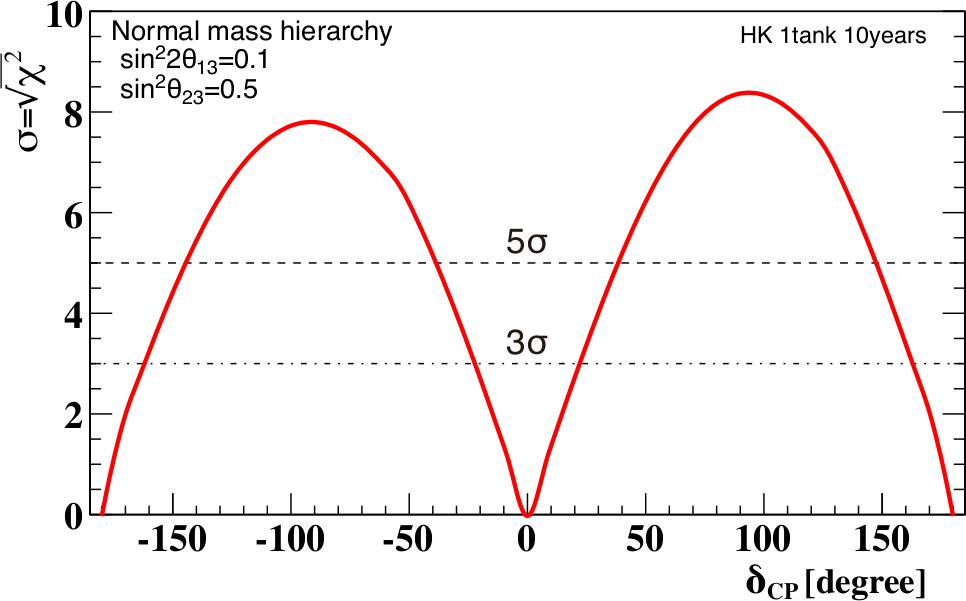
\includegraphics[width=\linewidth]{HKDRcpSens.png}
		\captionof{figure}{Expected significance to exclude CP conservation, %
			in case of normal hierarchy, where the mass hierarchy is assumed to be known~\cite{Abe:2018uyc}.}
		\label{fig:hkdr}
	\end{minipage}
\end{figure}


Given the parametrisation in Eq.~\ref{eq:pmns}, %
this asymmetry is not measurable if the phase is trivial, \ie~$\delta_\text{CP} = 0$~or~$\pm \pi$, %
or if $\theta_{13}$ is vanishing.
From a model building point of view, however, a successful leptogenesis requires the parameters to satisfy %
$\qty|\sin\theta_{13} \sin\delta_\text{CP}| \gtrsim 0.09$
%\begin{equation}
%	\label{eq:leptogenesis}
%	\qty|\sin\theta_{13} \sin\delta_\text{CP}| \gtrsim 0.09\ ,
%\end{equation}
when the Majorana phases are vanishing~\cite{Pascoli:2006ci}.
The value of $\theta_{13}$ has been measured to be non-zero~\cite{Abe:2011sj,Abe:2011fz,An:2012eh,Ahn:2012nd} %
and for this reason it is expected that on-going and future generation neutrino experiments %
will also constrain the value of $\delta_\text{CP}$.



\section{Hyper-Kamiokande experiment}

Hyper-Kamiokande (HK)~\cite{Abe:2018uyc} will be the next-generation water Cherenkov detector, %
superseding its predecessor, Super-Kamiokande (SK).
Employing ring-imaging technique, the rare interactions of neutrinos can be detected, %
as well as the possible spontaneous decay of nucleons.
The design of HK does not deviate much from SK and Kamiokande.
The cylindrical tank of HK will be 72\,m high and 68\,m in diameter, with a fiducial volume of 188.4\,kton (total volume 257.8\,kton), %
around 8.4 times the fiducial volume of SK.
The photo-coverage of the inner detector region will be 40\,\%, the same of SK, %
but it translates to roughly forty thousands photomultipliers (PMTs).
New 20''box and line PMTs will be employed, with improved charge and riming resolution, thanks to the increased quantum efficiency %
which is almost twice the QE of previous PMT generation.
It also has the high pressure tolerance for the usage below 60 m depth of water.
A study for implementing multi PMT modules, containing each 23 3'' PMT, is being carried out
The detector will be located underground at Kamioka mine in Gifu Prefecture, %
with an overburden of approximately 650 meters or more of rock, which is equivalent to \np{1750} meters or more of water.

Thanks to incredible statistics and cutting edge resolutions, HK will be capable of a vast variety of physics studies, %
from accelerator and atmospheric neutrinos to solar and supernova neutrinos.
Besides detecting proton decay, the main goal of HK is to measure~$\delta_\text{CP}$ and constrain the other oscillation parameters %
with high precision.
This is achievable by studying accelerator neutrinos, and to this end the possibility of installing a second detector in Korea, %
at the secondary oscillation peak, is being investigated.

HK will be located 295\,km away from the target and $2.5^\circ$ off-axis with respect to the beamline.
The detector cavity is planed to be excavated in Mt. Nijugo-yama in the Tochibora-mine in Gifu Prefecture, %
which is approximately 8\,km south from SK.
The neutrino beam is generated by a 30\,GeV proton beam colliding on a fixed graphite target; %
a`focusing horn selects positively charged ($\nu$ mode) or negatively charged ($\cj{\nu}$ mode) pions, %
which decay leptonically, to obtain an almost pure muon neutrino or antineutrino beam, peaking at 600\,MeV.
The accelerator facility at J-PARC will undergo a planned upgrade to increase the beam power up to 1.3\,MW, %
before HK starts operation.
The T2K near detector system, comprised of the two modules ND280 and INGRID, will be refurbished %
and the new Intermediate Water Cherenkov Detector, possibly gadolinium-loaded, will be located %
around 1\,km from the target.

HK will take data for ten years, collecting a total of \np{2.7e22} Protons On Target, %
divided between $\nu$ and $\cj{\nu}$ beam modes.
Studies have shown that CP violation discovery is not very sensitive to the time ratio between the two modes (ref?).
Assuming $\nu:\cj{\nu} = 1:3$ and $\delta_\text{CP} = 0$, %
the expected number of fully-contained events in the fiducial volume for the channels %
$\nu_\mu \to \nu_e$ and $\cj{\nu}_\mu \to \cj{\nu}_e$ %
are respectively \np{1643} and \np{15} in $\nu$ mode and \np{206} and \np{1183} in $\cj{\nu}$ mode, %
assuming CP conservation.
Deviations from these expected numbers could be indication of CP violation.
A preliminary study for the HK design report~\cite{Abe:2018uyc}, using a different analysis, %
estimated a significance well-above $5\,\sigma$ after ten years of data taking, as can be seen in Fig.~\ref{fig:hkdr}.

The project has been recentely approved by japanese goverment and data taking is expected commencing by 2027.

The uncertainty of the Earth’s density between Tokai and Kamioka is estimated to be at most 6\% [181].
Because the matter effect contribution to the total $\nu_\mu \to \nu_e$ appearance probability is %
less than 10\% for 295km baseline, the uncertainty from the matter density is estimated to be less
than 0.6\% and neglected in the following analysis.


\section{Sensitivity studies}

At any stage of the experiment it is important to asses the impact of systematic errors on the total sensitivity of HK.
One of the main goal is to constrain with high precision oscillation parameters, especially $\delta_\text{CP}$ and %
and the octant determination.
Even if real data is not available, it is possible to understand whether the statistics collected have %
enough constraining power to achieve the target precision.
The oscillation parameters and systematic uncertainties are input to a Monte Carlo simulation %
to build expected distribution of events.
This expected data is then compared to simulated \emph{observed data}, which is created by selecting %
a combination of oscillation parameters in order to mimic the real distributions of event that will be collected eventually.
Scanning over the oscillation parameters, the resolution of HK to oscillation parameters and, more importantly, %
the influence of the systematic uncertainties can be studied.
%To this end, a fitting framework is employed, capable of performing to study Monte Carlo simulation of beam and atmospheric samples. 

\subsection{Event samples}

\begin{table}
	\centering
	\caption{Samples event for atmospheric data. They are categorised as fully-contained sub-GeV (FC sub-GeV), %
		fully-contained multi-GeV (FC multi-GeV), partially-contained (PC) and upward-going muons (UP-$\mu$).}
	\label{tab:atmo_samples}
	\begin{tabular}{llcc}
		\toprule
		Event type	&	Sample	&	Bins $\log p$	& Bins $\cos\theta$  \\
		\midrule
		\multirow{7}{*}{\bf FC sub-GeV}	& one ring $e$-like and 0 decay-$e$	& 13 & 20 \\
						& one ring $e$-like and 1 decay-$e$	& 13 & 2 \\
						& one ring $\mu$-like and 0 decay-$e$	& 13 & 20 \\
						& one ring $\mu$-like and 1 decay-$e$	& 13 & 20\\
						& one ring $\mu$-like and 2 decay-$e$	& 13 & 2 \\
						& one ring $\pi^0$			& 13 & 2 \\
						& two rings $\pi^0$			& 5 & 2 \\
		\midrule
		\multirow{7}{*}{\bf FC multi-GeV}& one ring $\nu_e$-like     	& 10 & 20 \\
						& one ring $\cj{\nu}_e$-like    & 10 & 20 \\
						& one ring $\nu_\mu$-like       & 5 & 20 \\
						& multi ring $\nu_e$-like       & 8 & 20 \\
						& multi ring $\cj{\nu}_e$-like  & 8 & 20 \\
						& multi ring $\nu_\mu$-like     & 4 & 20 \\
						& multi ring other		& 10 & 20 \\
		\midrule
		\multirow{2}{*}{\bf PC}		& stopping 			& 4 & 20 \\
						& through-going 		& 5 & 20 \\
		\midrule
		\multirow{3}{*}{\bf UP-$\mu$}	& stopping 			& 4 & 20 \\
						& through-going, not showering 	& 1 & 20 \\
						& through-going, showering 	& 1 & 20 \\
		\bottomrule
	\end{tabular}
\end{table}

For the study, SK atmospheric Monte Carlo (MC) is adapted and scaled to HK statistics to compose the atmospheric sample.
A total of \np{2224} bins are used, divided in several two-dimensional histograms of $\log p$ and $\cos\vartheta$, %
where $\vartheta$ is the azimuthal angle.
These are divided in the usual categories of fully-contained, partially-contained, and upward-going muons, %
and are summarised in~\reftab{tab:atmo_samples}~\cite{Jiang:2019xwn}.
The beam sample, instead, is created using the far detector flux predicted with NEUT.
From the flux prediction, fully-contained candidate events in the fiducial volume are grouped %
as appeareance signal, i.e.\ $\nu_\mu\to\nu_e$ and $\cj{\nu}_\mu\to\cj{\nu}_e$, %
and background, i.e.\ unoscillated neutrinos.
Signal and background distributions in true energy (98 bins) undergo event selection criteria %
to obtain the distributions in reconstructed energy (87 bins) for the four event samples:
\begin{multicols}{2}
	\begin{itemize}
		\item one ring $e$-like in $\nu$-mode,
		\item one ring $\mu$-like in $\nu$-mode,
		\item one ring $e$-like in $\cj{\nu}$-mode,
		\item one ring $\mu$-like in $\cj{\nu}$-mode.
	\end{itemize}
\end{multicols}
A set of 2D smearing matrices, produced by the T2K fitting framework VALOR, %
simulates and replaces the correct event selection process, including tuning of the flux with near detector constraints.
These smearing matrices are provided for all samples, acting on signal (CCQE and CCnQE) %
and background (CCQE, CCnQE, and NC) distributions.

\begin{table}
	\centering
	\caption{Oscillation space.}
	\label{tab:osc_space}
	\begin{tabular}{cccc}
		\toprule
		Parameter				& Nominal	& Range	& Points \\
		\midrule
		$\Delta m_{12}^2/\np{e-5}\,\text{eV}^2$	& 7.53		& --			& fixed	\\
		$\sin^2 2\theta_{12}$			& 0.8463	& --			& fixed	\\
		\midrule
		$\Delta m_{23}^2/\np{e-3}\,\text{eV}^2$	& 2.509		& [2.464:2.554]		& 13	\\
		$\sin^2 2\theta_{13}$			& 0.085		& [0.070:0.100]		& 13	\\
		$\sin^2 \theta_{23}$			& 0.528		& [0.426:0.579]		& 19	\\
		$\delta_\text{CP}$			& $-\pi/2$	& [$-\pi$:$\pi$]	& 61	\\
		\bottomrule
	\end{tabular}
\end{table}


\subsection{Systematic model}

There are 67 systematics for the atmospheric sample, adopted from SK atmospheric studies~\cite{Abe:2017aap}.
List systematics.
A more accurate systematic study for the atmospheric analysis of HK is expected in the future.
The atmospheric systematics are initally uncorrelated with the beam systematics.
The focus of this work is the beam sample.

For the beam part, the T2K 2018 error model is employed~\cite{Abe:2018wpn}.
There are 74 uncertainties for flux and cross-section parameters, from near detector constraints, %
known as the BANFF fit. %
divided in $25\times 2$ systematics, for each beam mode, for the four main flux components, %
They are grouped in 50 systematics---25 for the $\nu$ mode and 25 for the $\cj{\nu}$~mode---%
for the main flux components ($\nu_e$, $\nu_\mu$, $\cj{\nu}_e$, and $\cj{\nu}_\mu$), % 
and 24 systematics for cross-section parameters.
There are also 45 uncertainties for SK detector efficiencies and Final State Interactions,
which parameterise the uncertainties on the four final state event selections at the far detector: %
1 ring $e$-like and 1 ring $\mu$-like in both $\nu$ and $\cj{\nu}$ modes.
The 1 ring $e$-like + 1 electron decay sample is not treated in this study.
Among these, one systematic describes the energy scale uncertainty.
It consists of 25 systematic uncertainities, constrained by near detector fits, for each beam mode---neutrino or antineutrino---describing %
are described by 25 systematics for each beam mode---neutrino or antineutrino.
There are 24 errors that describe cross section parameters, also constrained by near detector data.
from flux and cross-section parameters constrained by near detector fits.
Among the flux and cross-section parameters, These For the four main flux components 
25 uncertainties for the beam in neutrino mode and 25 for the antineutrino mode.
($2p2h$ normalisation and shape for \tapi{16}O, CCQE axial-mass scaling factor, CC and NC interaction normalisations, %
RPA coefficients, binding energy on oxygen).
In addition, there are 45 systematics from SK detector efficiencies and Final State Interactions, %
which parameterise the uncertainties on the four final state interaction types %
at the far detector: %
1 ring $e$-like and 1 ring $\mu$-like in both $\nu$ and $\cj{\nu}$ modes.
One systematic is adopted to describe the energy scale uncertainty at the far detector.

The momentum reconstruction of neutrino event is mainly based on the charge observed
by the PMTs in the tank. The factors discussed above, including water property or
PMT gain will affect the performance of momentum reconstruction. On the other hand,
the precise momentum determination of the neutrino event is necessary for the neutrino
oscillation analysis since the oscillation probability is highly related to the energy of
neutrinos. Four well-known independent control samples are used for the energy scale
calibration [6] and systematic evaluation in different momentum range:
Track length of high energy stopping muons (1 -- 10 GeV/c)
Cherenkov angle of low energy stopping muons (200 -- 500 MeV/c)
Invariant mass of $\pi^0$ produced by neutrino interactions (-- 130 MeV/c)
Momentum distribution of decay electron (-- 40MeV/c).

\subsection{Oscillation space}

Both the atmospheric and beam distributions are weighted by the corresponding oscillation probabilities.
For the study of this thesis, the oscillation parameters are scanned over the space
The oscillation space spans four variables, $\Delta m^2_{32}$, $\sin^2 2\theta_{13}$, $\sin^2 \theta_{23}$, and %
$\delta_\text{CP}$, on a grid of respectively $13\,\times\,13\,\times\,19\,\times\,61$ points.
The solar squared mass difference and the solar angle are fixed.
Apart from $\delta_\text{CP}$ which is scanned over all possible values, %
the intervals for the other parameters are built around ``Asimov A'', the nominal T2K best fit point~\cite{Abe:2017vif} .
For the atmospheric squared mass difference and the reactor angle, the range is chosen such that it covers %
a $[-3\sigma, +3\sigma]$ interval, where $\sigma$ is the error from the Asimov A set; %
the range for $\sin^2\theta_{23}$ spans over $[-6\sigma:+3\sigma]$ so that both octants are covered.
Reactor experiments~\cite{Bak:2018ydk, Adey:2018zwh}.
At each point of this space, the event distributions are weighted with the correct oscillation probability %
for appearance or disappearance channels.
A special point of the parameter space is chosen as a \emph{true} combination of oscillation parameters %
to perform sensitivity studies using a $\chi^2$-test statistics.
By changing the \emph{true} point, it is possible to define the exclusion regions for CP violation, %
by comparing the $\chi^2$ at any value of $\delta_\text{CP}$ with the $\chi^2$ computed at %
the null hypothesis, i.e.\ CP conservation.
The sensitivity to exclude the $\sin \delta_\text{CP} = 0$ as a function of \emph{true} $\delta_\text{CP}$ %
is quantified by %
\begin{equation}
	\sigma = \sqrt{\min_{\delta_\text{CP} = 0,\pm\pi}\! \chi^2\  -\,\chi^2_\text{\emph{true}}}\ ,
\end{equation}
where $\chi^2_\text{\emph{true}}$ is evaluated at the \emph{true} point.

\subsection{$\chi^2$ test}

The test statistics of this analysis is defined as a ``pull approach'' $\chi^2$~\cite{Fogli:2002pt}, in the following way
%\begin{align}
%	\chi^2_\text{tot} &=\ \chi^2_\text{obs}\ +\ \chi^2_\text{syst} \notag\\
%	&= \overset{\text{obs}}{2 \sum_n \qty[E_n(1+{\textstyle\sum_j f_j^n \varepsilon_j}) - O_n + O_n \log \qty(\frac{E_n(1+\sum_j f_j^n \varepsilon_j)}{O_n})]} + %
%	\overset{\text{\shortstack{syst\\ \hphantom{.}}}}{\sum_{ij} \varepsilon_i\, \rho^{-1}_{ij}\, \varepsilon_j}\ ,
%\end{align}
\begin{equation}
	\chi^2 = \min_{\uj{\varepsilon}}\, \qty\Big[\,\chi^2(\vartheta;\uj{\varepsilon})\,]\ ,
\end{equation}
with $\vartheta$ the oscillation parameters and $\uj{\varepsilon}$ the full set of $j$ systematic errors, and
\begin{equation}
	\label{eq:chi2}
	\chi^2(\vartheta;\uj{\epsilon})  = 2 \sum_n \qty[E_n(1+{\textstyle\sum_j f_j^n \varepsilon_j}) - O_n + %
		O_n \log \qty(\frac{E_n(1+\sum_j f_j^n \varepsilon_j)}{O_n})] + %
		\sum_{ij} \varepsilon_i\, \rho^{-1}_{ij}\, \varepsilon_j\ ,
\end{equation}
where $O_n$ and $E_n$ are respectively the number of observed and expected events in the $n$-th bin and~$\rho^{-1}$ %
is the inverse of the correlation matrix of the systematic errors.
As there is no real data, the ``observed'' events are replaced by a prediction at the \emph{true} oscillation point.
The systematic uncertainties are embedded in the $f_j^n$ term, which is the fractional change %
induced on the $n$-th bin by a 1\,$\sigma$ variation of the $j$-th systematic;
the amount of the shift is quantified by the ``pull'' $\varepsilon_j$ in units of the uncertainty $\sigma_j$.
For most of the systematic parameters, a linear response is assumed in the~MC.
This means that varying of the $j$-th systematic by a known amount, $\beta_j \to \beta_j + \varepsilon_j\sigma_j$, %
the number of expected events changes:
\begin{align*}
	\beta_j\ \overset{\scriptstyle \text{MC}}{\longmapsto}\ E_n %
	%\qquad \overset{\varepsilon_j \sigma_j}{\Longrightarrow} \qquad %
	\qquad \Longrightarrow \qquad %
	\beta_j + \varepsilon_j\sigma_j\ \overset{\text{MC}}{\longmapsto}\ E_n ( 1 + \varepsilon_j f_n ^j )\ .
	%&\hspace{0.4em}\text{\scriptsize MC} \\
	%\text{\scriptsize MC\ :} \hspace{1em} \Downarrow & \hspace{3.5em} \Downarrow	\\	
\end{align*}
Certain systematic uncertainties, such as the CCQE axial-mass scaling factor, the Fermi momentum for \tapi{16}O, %
or some of the RPA coefficients\footnote{The Random Phase Approximation (RPA) method is applied to calculate the total cross sections %
	of electron neutrinos on nuclei.}, 
do not present a linear behaviour for small values of $\varepsilon$ %
and they are better described by a four-point linear interpolation of different~$f_j^n$ histograms, %
computed at~$\pm1\,\sigma$ and~$\pm3\,\sigma$ variations of the systematic parameter.
Given a \emph{true} point, the $\chi^2$ is computed at each point of the oscillation parameter space %
and it is minimised with respect to the pulls $\varepsilon$.
This leads to a set of $j$ non-linear equations %, which can be solved iteratively if the condition $\sum_j f^n_j \varepsilon_j < 1$~holds.
\begin{equation}
	\pdv{\chi^2}{\varepsilon_j} (\vartheta;\uj{\varepsilon}) = 0\ .
\end{equation}
The system can be solved with the Newton's method by finding the Hessian of the $\chi^2$.
This gives a linear system, which can be iterated until sufficient precision is achieved
\begin{equation}
	\pdv{\chi^2(\uj{\varepsilon}^{(n)})}{\varepsilon_k}{\varepsilon_j} %
	\cdot \qty(\varepsilon_j^{(n+1)} - \varepsilon_j^{(n)}) = %
	-\pdv{\chi^2(\uj{\varepsilon}^{(n)})}{\varepsilon_k}\ ,
\end{equation}
with $(n)$ the iteration index.
To account for future constraints from other experiments, a gaussian penalty terms is added %
to the $\chi^2$ definition of \refeq{eq:chi2}
\begin{equation}
	\chi^2_\text{penalty} = \frac{(\vartheta - \hat{\vartheta})^2}{\sigma_\vartheta^2}\ .
\end{equation}
The current constraint applied is the measurement of $\theta_{13}$ by future reactor experiments, %
that will achieve $\sin^2 2\theta_{13} = 0.085 \pm 0.005$.

\section{Systematic studies}

It is expected that larger systematic errors will result in a worse sensitivity,
but certain uncertainties affect the measurement of the oscillation parameters more than others.
For example, these can be the uncertainties on $\nu_e$ and $\cj{\nu}_e$ charged-current cross sections, %
the transverse flux model, the pion absorption probability, the total energy scale in SK, or the flux alignment.
We study the impact of some selected systematics by modifying the nominal systematic model %
and analysing the overall predicted sensitivity of the experiment in these different scenarios.
Doing so, it is possible to determine which systematics have the most important repercussion on the sensitivity,
since it is fundamental to understand their effect at all phases of the experiment.

\subsection{Validation of the fitter}

To validate the fitting framework a special systematic set for the beam sample is used.
It is composed of just two systematics: the $\nu_e$ and the $\cj{\nu_e}$ CC cross-section uncertainties.
These two errors are correlated, anti-correlated (and uncorrelated) %
and they are tested at different magnitudes: 1\%, 2\%, 3\%, 4\%, and 5\%.
This means a total of 15 fits.
Given the definition of $\chi^2$ in \refeq{eq:chi2}, %
at fixed magnitude the difference between the sets is just the correlation matrix, whereas at fixed correlation matrix %
the differencea are the $1\sigma$ histograms.
\begin{equation}
	\rho = \mqty(1 & 1 \\ 1 & 1) \quad,\quad
	\rho = \mqty(1 & -1 \\ -1 & 1) \quad,\quad
	\rho = \mqty(1 & 0 \\ 0 & 1)\ .
\end{equation}
The correlation matrices written as above are singular and so not invertible.
In order to get the inverted matrix, an offset of \np{e-5} is added to off-diagonal terms.

\subsection{Variations to the nominal model}

A series of modifications are performed on the nominal systematic model is modified:

\section{Dependencies on exclusion of CP}

Unknown mass hierachy, statistics ecc, octant determination.
